\documentclass[11pt,a4paper]{article}
\usepackage[T1]{fontenc}
\usepackage{lmodern,amsmath,amssymb,graphicx,booktabs,array}
\usepackage[margin=25mm]{geometry}
\usepackage{microtype}
\usepackage[colorlinks=true,linkcolor=blue,citecolor=blue,urlcolor=blue,breaklinks=true]{hyperref}
\hypersetup{pdftitle={Repeated Driving and Retained State in Early SRG Motion},pdfauthor={Hilmir Frimann Halldorsson},pdfsubject={SRG-SIM02 bounded paired continuation, v0.1}}
\graphicspath{{plots/}}
\setlength{\parskip}{4pt}
\setlength{\parindent}{1em}
\setlength{\emergencystretch}{1.5em}
\widowpenalty=10000
\clubpenalty=10000
\renewcommand{\arraystretch}{1.15}
\newcommand{\norm}[1]{\left\lVert #1\right\rVert}
\newcommand{\C}{\mathrm{C}}
\newcommand{\R}{\mathrm{R}}
\newcommand{\mi}{\mathcal M_{10}}
\newcommand{\wrap}{\mathcal W_{10}}
\title{\textbf{Repeated Driving and Retained State\\in Early SRG Motion}\\[5pt]
\large A Bounded Paired Continuation of Historical Engine C}
\author{Hilmir Fr\'imann Halld\'orsson}
\date{SRG-SIM02 \quad Version 0.1 \quad 14 October 2026}
\begin{document}
\maketitle
\begin{abstract}
Repeating a prescribed driving waveform need not repeat the state of the system it drives. We examine that distinction in an unchanged historical SRG numerical program, engine C, which moves eight labeled centers in a periodic three-dimensional box. The program retains positions, velocities and binary force signs, with sign toggles governed by a speed-dependent gate and a legacy pseudorandom stream. Two continuations inherit the same accepted 200-update prefix and full random-generator checkpoint. Each adds 800 updates. One supplies continuously increasing frame labels; the other repeats labels 0--199 while carrying all state forward. The repeated schedule renews substantial speed pulses: its four new block-average speeds lie between 0.09858 and 0.10503, whereas the continuous arm's block averages decrease from 0.008812 to 0.002106. The repeated waveform does not produce a tested same-phase labeled-state near-repeat. Positions and velocities diverge between arms at the first new successor, before the first new toggle. All new cross-arm draw values, their assignments and bit histories nevertheless match. A source-derived pre-damping increment identity helps explain how similar magnitude envelopes can coexist with changing directions and configurations. The result is a finite response to a changed driving schedule, conditional on one inherited state and realized stream; it establishes neither learned memory nor an asymptotic attractor. No new scientific execution was performed to prepare this paper.
\end{abstract}

\section{A repeated clock input and a continuing state}
\label{sec:question}
An animation can revisit a frame label without restoring the numerical state associated with the earlier visit. In a stateful numerical program, those are different operations. A repeated label can renew a prescribed input while positions, velocities and other carried variables continue from their current values. The scientific question is then concrete: what repeats in the response, and what continues to change?

The accepted SIM01 reconstruction identified this distinction in a surviving family of early SRG motion programs. In that family, historical frame labels can restart while state persists. SIM01 selected engine C as the base for studying the family's explicit feedback and retained binary signs, and supplied a finite 200-update C record and complete continuation checkpoint~\cite{sim01}. SIM02 used that accepted checkpoint to compare two supplied-frame schedules without replacing C's numerical operator~\cite{sim02}. It does not reconstruct an unknown history of GUI invocations.

This paper explains the completed SIM02 experiment and its subsequent GPT-assisted scientific review. Its main result combines three observations: renewed speed under repeated driving, changing labeled states at corresponding driving phases, and exactly matched realized randomness between the arms at equal actual update counts~\cite{sim02,review}. The third observation is particularly informative because it rules out random-stream mismatch as an explanation of the observed cross-arm separation in this realization. It does not remove C's stochastic rule or isolate the contribution of each carried variable.

The scope is the surviving motion program and this bounded continuation. The unidentified June topology producer, other SRG mathematical constructions and physical calibration questions remain outside the study. SRG is treated here as an independent mathematical and computational research program; no correspondence with an established physical dynamics is assumed.

\section{The unchanged numerical model}
\label{sec:model}
\subsection{State, labels and periodic coordinates}
C carries eight labeled centers, indexed by $i=0,\ldots,7$, with positions $p_i\in[0,10)^3$, velocities $v_i\in\mathbb R^3$ and retained bits $b_i\in\{0,1\}$. The reproducible continuation state also includes the complete legacy NumPy MT19937 state, denoted $\rho$. Write
\begin{equation}
 S=(p_0,\ldots,p_7;\ v_0,\ldots,v_7;\ b_0,\ldots,b_7;\ \rho).
 \label{eq:state}
\end{equation}
The generator checkpoint contains its 624 keys, position and Gaussian-cache fields. A seed alone is not a substitute for the saved continuation checkpoint. The supplied frame $f$ is an input to the next call, separate from the count of calls already completed. The tetrahedra in the historical display are attached shapes; this engine has no independent rotational or deformational state for them~\cite{sim01,source}.

For vectors, wrapping and the minimal-image convention act componentwise:
\begin{equation}
 \wrap(x)=x\bmod 10,\qquad \mi(x)=((x+5)\bmod10)-5.
 \label{eq:wrap}
\end{equation}
The first chooses stored coordinates in $[0,10)$; the second chooses signed coordinate differences in $[-5,5)$. C uses an arithmetic centroid of the currently stored wrapped coordinates, not a circular or intrinsic torus centroid. The choice is part of the historical operator. Replacing it would define a different experiment~\cite{source}.

\subsection{Prescribed driving, incoming feedback and damping}
The source time is $t=0.1f$, with $\Delta t=\mathrm{DT}=0.1$. The prescribed driving function is
\begin{equation}
 H(t)=2e^{-0.5t}\cos t+e^{-0.3t}\sin t+1.5e^{-0.7t}+e^{-0.4t}.
 \label{eq:H}
\end{equation}
In particular, $H(0)=4.5$. The source calls this a memory curve, but it is evaluated from the supplied time; it is not accumulated from the trajectory. The common feedback factor, called GRF in the program, is
\begin{equation}
 G(S)=\frac{1}{1+u(S)},\qquad u(S)=\frac18\sum_{i=0}^7\norm{v_i}.
 \label{eq:G}
\end{equation}
It is evaluated from the incoming velocities once per complete eight-center call and remains frozen throughout that call. Damping, called RPCO, acts on each velocity component:
\begin{equation}
 D(w)_a=\frac{w_a}{1+\log(1+|w_a|)},\qquad a=1,2,3.
 \label{eq:damp}
\end{equation}
The actual executable uses \texttt{np.log1p}, not a substituted logarithm expression. Equations~\eqref{eq:H}--\eqref{eq:damp} describe the source in real-valued notation. Their use below does not assert equality of all algebraically rearranged floating-point implementations~\cite{source}.

\subsection{One call, in source order}
\label{sec:order}
Let $p^{[i]}_\ell$ denote the stored position of center $\ell$ immediately before center $i$ is visited during a call. Centers $\ell<i$ have already moved; centers $\ell\geq i$ have not. With $G$ and $H(t)$ fixed for the call, the sequential geometry is
\begin{align}
 c^{[i]}&=\frac18\sum_{\ell=0}^7p^{[i]}_\ell,
 & d_i&=\mi\!\left(c^{[i]}-p_i^{[i]}\right),
 & r_i&=\norm{d_i}+0.01.
 \label{eq:centroid}
\end{align}
The regularizer $0.01$ is added to the norm. Before calculating that center's force sign, C applies its gated toggle rule. If $G>0.5$, it consumes exactly one scalar native draw $U_i=\texttt{np.random.rand()}$. On this open gate,
\begin{equation}
 b_i^+=\begin{cases}1-b_i,&U_i<0.01,\\ b_i,&U_i\geq0.01.\end{cases}
 \label{eq:toggle}
\end{equation}
If $G\leq0.5$, it consumes no draw and leaves $b_i$ unchanged. Short-circuit evaluation is therefore part of the generator semantics. No dummy value is consumed on a closed gate.

The selected sign is $s_i=+1$ for $b_i^+=0$ and $s_i=-1$ for $b_i^+=1$. The remaining operations are, in source order,
\begin{align}
 F_i&=\frac{d_i}{r_i}\,H(t)\,s_i,\label{eq:force}\\
 w_i&=v_i+\Delta t\,F_i\,G,\label{eq:predamp}\\
 v_i^+&=D(w_i),\label{eq:velocity}\\
 p_i^+&=\wrap\!\left(p_i+\Delta t\,v_i^+\right).\label{eq:position}
\end{align}
The new $p_i^+$ is stored before the next centroid is calculated. G is not recomputed at that point. The bit update precedes the force, and the damped velocity precedes the position increment. These details distinguish C from a simultaneous-center scheme or a different stochastic update order~\cite{source}.

SIM02 used exact-byte copies of the accepted detached core and its observation API. It preserved the original scalar arithmetic, expression grouping, sequential order, gate and draw consumption. The wrapper provided schedules, restoration and logging; it did not introduce another engine. The kinetic-like and displacement diagnostics discussed in Section~\ref{sec:observer} are observers and do not feed back into Eqs.~\eqref{eq:force}--\eqref{eq:position}~\cite{sim02,review}.

\section{The matched-prefix experiment}
\label{sec:design}
Let $S_k$ be the state after $k$ complete updates. Actual update $n$ takes $S_n$ to $S_{n+1}$. The accepted prefix consists of updates $0,\ldots,199$ and states $S_0,\ldots,S_{200}$. Each arm restored exactly the same $S_{200}$ and full final generator checkpoint, then executed updates $200,\ldots,999$ once~\cite{sim02}.

\begin{table}[htbp]
\centering\small
\begin{tabular}{lll}
\toprule Arm & Supplied frame at actual update $n$ & Source time \\
\midrule CONTINUOUS & $f_n=n$ & $0.1n$ \\
REPEATED & $f_n=n\bmod200$ & $0.1(n\bmod200)$ \\
\bottomrule
\end{tabular}
\caption{The sole schedule intervention. Both arms retain the same inherited prefix. REPEATED restarts only the supplied frame at $n=200,400,600,800$; positions, velocities, bits and RNG state continue. Source: accepted SIM02 specification and report~\cite{sim02}.}
\label{tab:schedule}
\end{table}

Each new continuation contains 801 states $S_{200},\ldots,S_{1000}$ and 800 per-update records. A joined view uses the inherited prefix once and has 1,001 states and 1,000 updates, with no duplicate $S_{200}$. There is no update $n=1000$. The common first block is one inherited observation reused in two views, not two independently executed prefixes~\cite{sim02}.

The saved prefix serializes bits as \texttt{int8}. The accepted restoration first validated the binary values, then widened them losslessly to C's original \texttt{dtype=int}, which was \texttt{int64} in the execution environment. Positions and velocities were restored as independently owned, writable, C-contiguous \texttt{float64} arrays. The complete MT19937 state round-tripped without a test draw~\cite{sim02,review}.

Before rollout, four isolated disposable calls compared observed and unobserved successors from the pristine branch: one pair at frame 200 and one at frame 0. Each pair agreed bitwise in positions and velocities, in bit values and dtypes, and in metadata and complete post-call RNG state. The observed traces also checked sequential center order and passive diagnostic preservation. The rollout processes restored the pristine checkpoint again; no preflight successor became a rollout input~\cite{sim02,review}.

The completed execution budget was $4+800+800=1{,}604$ calls started and completed. The two arms ran in separate serial processes, avoiding a shared process-global RNG between arms. No inherited update was rerun, and no state or RNG reset occurred at a cycle boundary. These are facts of the accepted execution, not work newly performed to produce this manuscript~\cite{sim02}.

\section{Readouts and comparison conventions}
\label{sec:measure}
Mean speed is $u(S)$ in Eq.~\eqref{eq:G}. It averages speed magnitudes, not velocity vectors. Mean periodic pair separation averages 28 unordered pairs:
\begin{equation}
 q(S)=\frac1{28}\sum_{0\leq i<j\leq7}\norm{\mi(p_i-p_j)}.
 \label{eq:pair}
\end{equation}
For two states $S,T$ at equal actual update count, define labeled-center residuals
\begin{equation}
 a_i(S,T)=\norm{\mi(p_i(S)-p_i(T))},\qquad
 z_i(S,T)=\norm{v_i(S)-v_i(T)}.
 \label{eq:residual}
\end{equation}
We report $\overline a$, $\max_i a_i$, $\overline z$ and $\max_i z_i$ separately, together with the bit Hamming count
\begin{equation}
 h_b(S,T)=\sum_{i=0}^7\mathbf1\{b_i(S)\ne b_i(T)\}.
 \label{eq:hamming}
\end{equation}
These compare corresponding labels. They do not optimize over rotations or permutations and are not a composite complexity measure~\cite{sim02,records}.

For REPEATED, write $n=200c+j$, with cycle $c=0,\ldots,4$ and phase $j=0,\ldots,199$. The sampled post-update responses are
\begin{equation}
 u_{c,j}=u(S_{200c+j+1}),\qquad q_{c,j}=q(S_{200c+j+1}).
 \label{eq:phase}
\end{equation}
In contrast, $G_{c,j}$ is computed from the incoming state $S_{200c+j}$, and $H_{c,j}$ belongs to update $200c+j$. Boundary incoming states are $S_{200c}$, with $S_{1000}$ the final boundary. This distinction matters when comparing a velocity response with the feedback used to generate it.

The declared geometric/bit near-repeat diagnostic requires
\begin{equation}
 \overline a,\ \max_i a_i,\ \overline z,\ \max_i z_i\ \leq 10^{-12},
 \qquad h_b=0.
 \label{eq:near}
\end{equation}
The inequalities are in native coordinate and velocity units. This tolerance is an operational convention, not a physical resolution. Passing it would still not establish recurrence of the complete state in Eq.~\eqref{eq:state}, since the RNG state also matters. The accepted comparisons include successive cycles and each later cycle against inherited cycle 0~\cite{sim02,review}.

\section{Renewed motion under the repeated schedule}
\label{sec:speed}
At actual update 200, the arms have the same incoming $G=0.9853316764949968$. Their driving values differ immediately: CONTINUOUS uses $H=0.002636728742286805$, whereas REPEATED uses $H=4.5$. The schedule intervention therefore renews a much larger input before the first new successor is saved~\cite{sim02,review}.

\begin{figure}[htbp]
\centering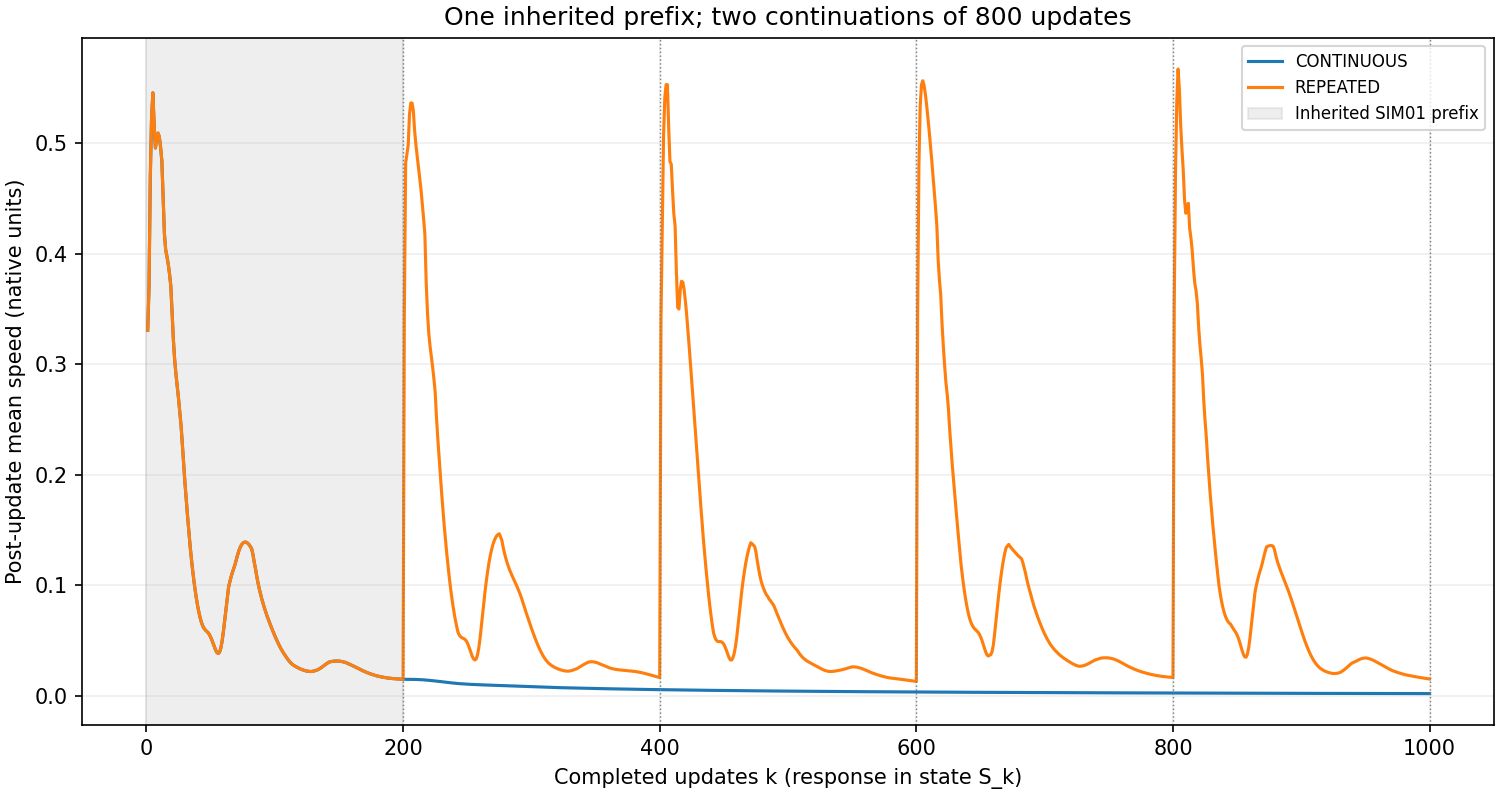
\includegraphics[width=\linewidth]{01_mean_speed.png}
\caption{Accepted mean-speed record versus actual completed updates $k$, so the plotted response belongs to $S_k$. The shaded first 200 updates are the single inherited cycle 0, shared by both views. The four later blocks are new; only REPEATED restarts its supplied frame at the marked boundaries. The original image is unchanged~\cite{sim02,records}.}
\label{fig:speed}
\end{figure}

Figure~\ref{fig:speed} shows the resulting renewed pulses. Table~\ref{tab:means} summarizes the new blocks only. CONTINUOUS has successively lower block-average speed, while REPEATED maintains averages near 0.10 without a monotone sequence of block means. These are averages of the 200 post-update mean speeds in each block~\cite{records,reviewdata}.

\begin{table}[htbp]
\centering\small
\begin{tabular}{rrr}
\toprule Actual update indices & CONTINUOUS mean speed & REPEATED mean speed \\
\midrule
200--399 & 0.008811537 & 0.103946551 \\
400--599 & 0.004189443 & 0.098578750 \\
600--799 & 0.002796353 & 0.105028978 \\
800--999 & 0.002105524 & 0.100533001 \\
\bottomrule
\end{tabular}
\caption{Four new block averages; the inherited block is excluded. Values are rounded from accepted saved readouts, also checked in the subsequent review~\cite{records,reviewdata}.}
\label{tab:means}
\end{table}

The five repeated phase curves share an exactly equal sampled $H$ waveform, but their speed curves are not identical. Their common broad envelope includes a large early pulse and smaller later features (Fig.~\ref{fig:phase-speed}). The inherited cycle's peak is about 0.545645; the new peaks are 0.536404, 0.553068, 0.556542 and 0.567208. Similar scalar envelopes are a descriptive observation, not a synchronization or convergence theorem~\cite{records,reviewdata}.

\begin{figure}[htbp]
\centering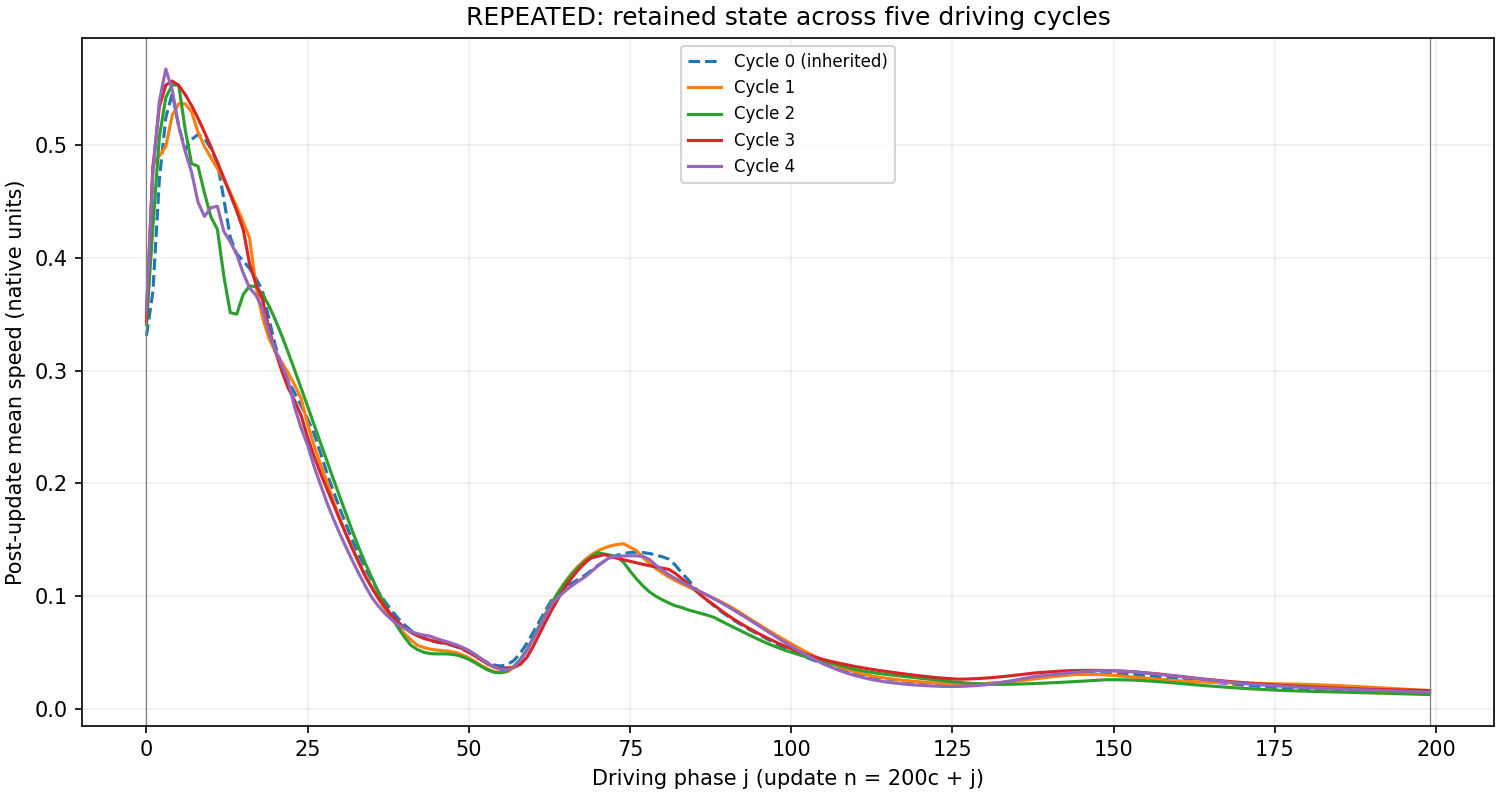
\includegraphics[width=\linewidth]{04_repeated_speed.png}
\caption{Accepted REPEATED speed versus driving phase $j$. The dashed curve is inherited cycle 0; cycles 1--4 are newly executed. Every response is post-update, in $S_{200c+j+1}$. Similar envelopes coexist with different labeled states; the curves are not independent repeated trials. The original image is unchanged~\cite{sim02,records}.}
\label{fig:phase-speed}
\end{figure}

At $S_{1000}$, mean speeds are 0.001868639754721557 and 0.015128603885987843 in CONTINUOUS and REPEATED respectively. This endpoint samples the weak-driving end of the repeated cycle, rather than its renewed peak. The result should therefore be read together with the block averages and phase curves, not compressed into a single performance score~\cite{records,reviewdata}.

\section{Changing geometry and feedback}
\label{sec:geometry}
Mean pair separation does not follow a monotone contraction across the repeated cycles. It decreases through the early cycles and rises later (Figs.~\ref{fig:pair} and \ref{fig:phase-pair}). Table~\ref{tab:cycle} compares cycle-average separation and G with the endpoint speed. The same driving waveform can accompany different configurations and different feedback within this horizon~\cite{records}.

\begin{figure}[htbp]
\centering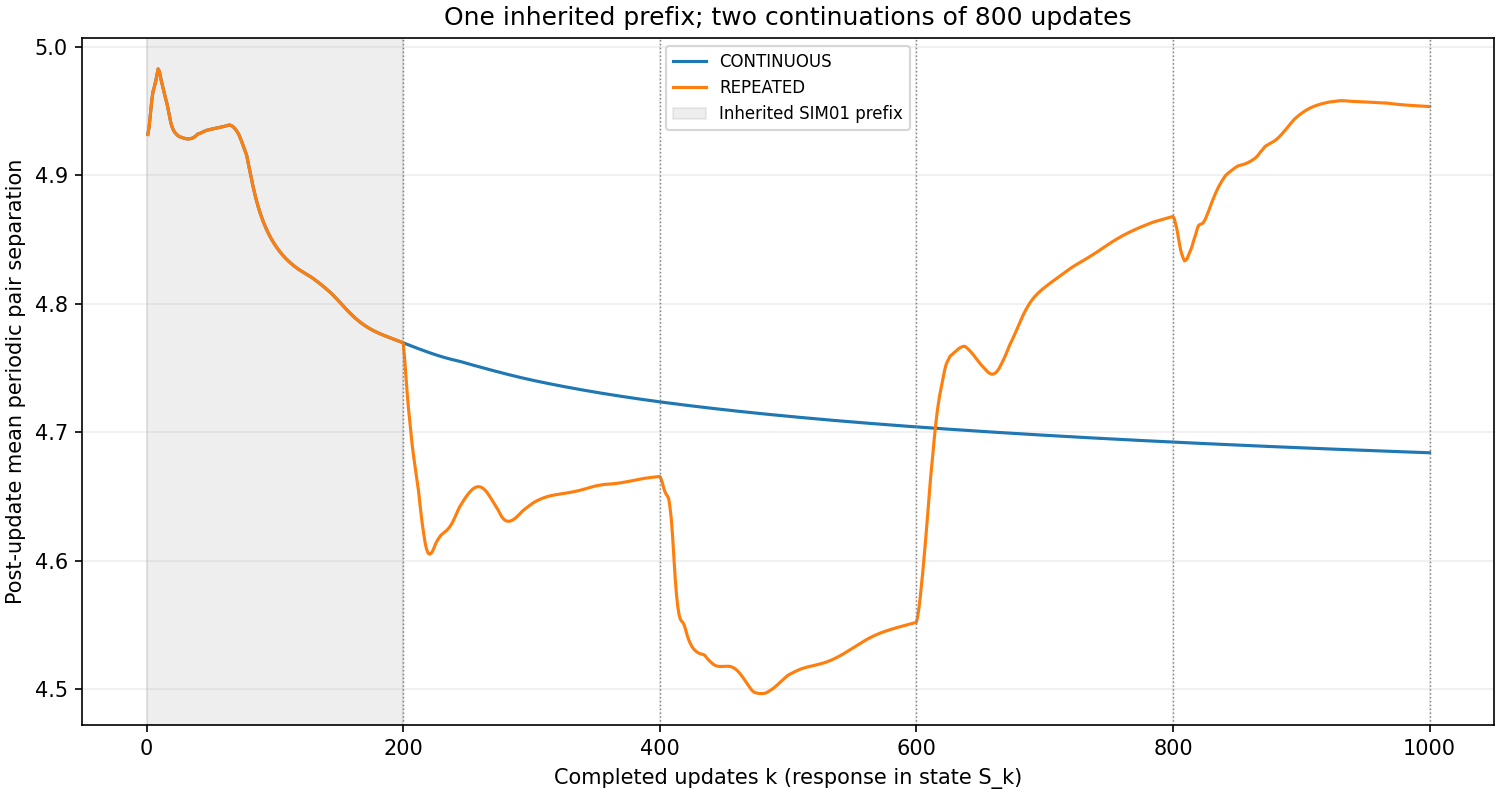
\includegraphics[width=\linewidth]{02_pair_separation.png}
\caption{Accepted periodic pair separation versus completed updates $k$, evaluated in post-update state $S_k$. The shaded first block is the shared inherited cycle 0; the later four are new. Dotted boundaries identify repeated-frame resets only for REPEATED. No circular-centroid replacement or shape alignment was applied. The original image is unchanged~\cite{sim02,records}.}
\label{fig:pair}
\end{figure}

\begin{table}[htbp]
\centering\small
\begin{tabular}{rrrrr}
\toprule Repeated cycle & Mean $q$ & Last $q$ & Mean incoming $G$ & Last speed \\
\midrule
0 (inherited) & 4.863220 & 4.769511 & 0.917109 & 0.014887 \\
1 & 4.650320 & 4.665506 & 0.916755 & 0.016337 \\
2 & 4.531935 & 4.551918 & 0.920646 & 0.012879 \\
3 & 4.795444 & 4.867813 & 0.915984 & 0.016438 \\
4 & 4.926751 & 4.953356 & 0.918720 & 0.015129 \\
\bottomrule
\end{tabular}
\caption{Selected repeated-cycle readouts from the unchanged cycle summary~\cite{records}. The last $q$ and speed are at $S_{200(c+1)}$; mean incoming G averages updates $200c$ through $200c+199$. Full minima, maxima and first/last values remain in the accepted CSV.}
\label{tab:cycle}
\end{table}

The new-update G ranges are $0.9853316765$ to $0.9981328229$ for CONTINUOUS and $0.6380773618$ to $0.9872843536$ for REPEATED. Renewed speeds lower G substantially within the repeated cycles, while every recorded gate remains above 0.5. The two unchanged G figures are collected in Appendix~\ref{app:feedback}; they use incoming rather than post-update indexing~\cite{sim02,reviewdata}.

\begin{figure}[htbp]
\centering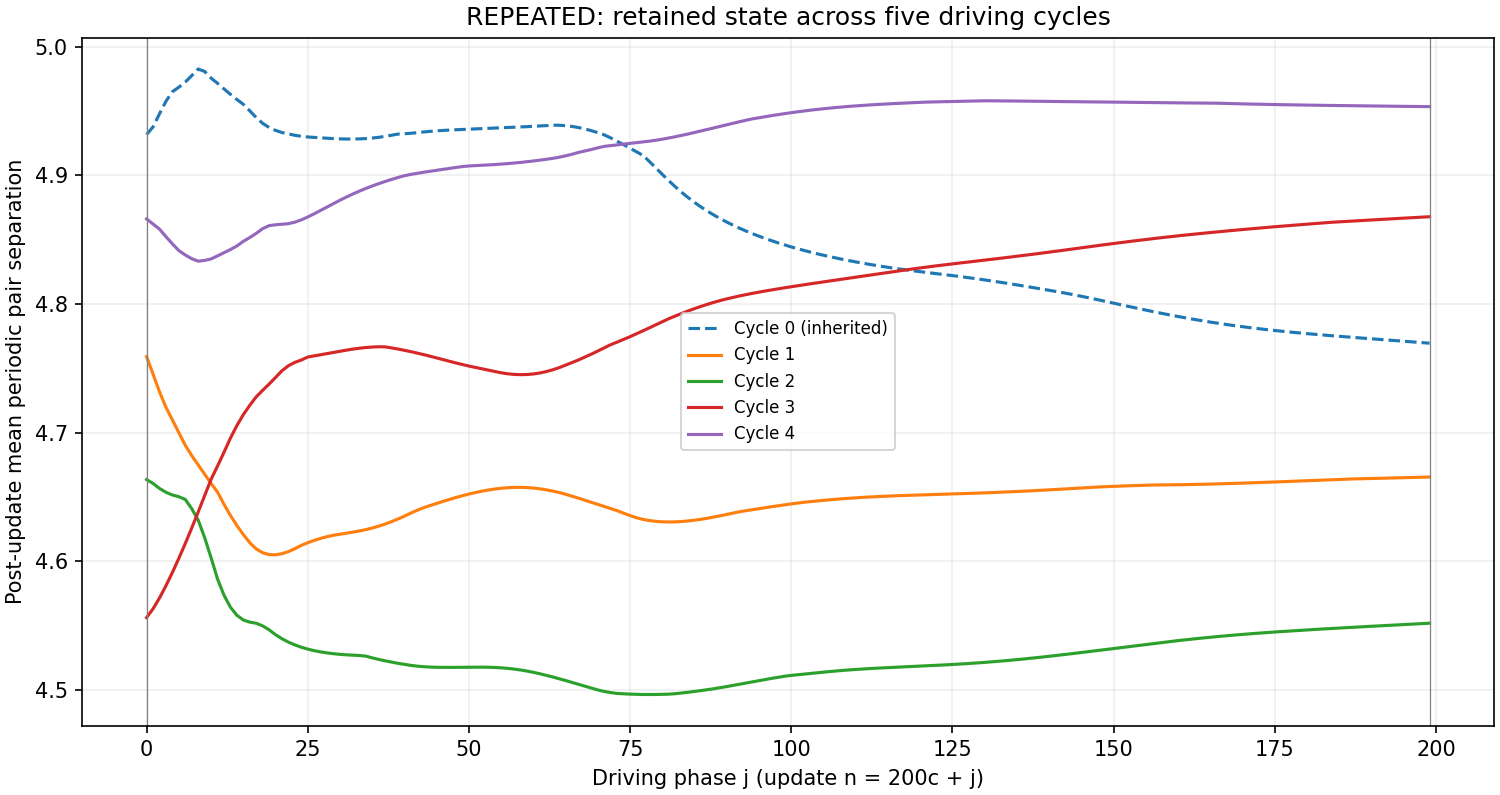
\includegraphics[width=\linewidth]{05_repeated_separation.png}
\caption{Accepted REPEATED pair separation versus phase $j$, measured in $S_{200c+j+1}$. Cycle 0 is inherited and dashed; cycles 1--4 are new. Each phase compares the same driving label while geometry and other carried state continue. The original image is unchanged~\cite{sim02,records}.}
\label{fig:phase-pair}
\end{figure}

Between arms, positions and velocities first differ at $S_{201}$. The mean labeled-center position residual grows across the four new 200-update boundaries listed in Table~\ref{tab:cross}, while the bits remain equal. At the final boundary the largest centerwise position residual is about 6.573548; it is a three-dimensional minimal-image norm, not a single coordinate difference~\cite{records,reviewdata}.

\begin{table}[htbp]
\centering\small
\begin{tabular}{rrrrrr}
\toprule State & $\overline a$ & $\max a_i$ & $\overline z$ & $\max z_i$ & $h_b$ \\
\midrule
$S_{200}$ & 0 & 0 & 0 & 0 & 0 \\
$S_{400}$ & 1.276737 & 2.096532 & 0.016633 & 0.024082 & 0 \\
$S_{600}$ & 1.825098 & 3.374302 & 0.014924 & 0.020714 & 0 \\
$S_{800}$ & 2.534526 & 5.108251 & 0.016701 & 0.022497 & 0 \\
$S_{1000}$ & 2.851058 & 6.573548 & 0.015897 & 0.019734 & 0 \\
\bottomrule
\end{tabular}
\caption{Cross-arm residuals at equal actual counts, using Eqs.~\eqref{eq:residual}--\eqref{eq:hamming}. Source: accepted \texttt{cross\_arm\_boundaries.csv}~\cite{records}. Position, velocity and bit results remain separate.}
\label{tab:cross}
\end{table}

\section{Matched draws and tested same-phase states}
\label{sec:randomness}
All 800 new gates were open in both arms. Each arm therefore consumed eight native scalar draws per update, in the same center order, from the same restored checkpoint. The accepted record and subsequent review find exact agreement of all 6,400 cross-arm draw values and their assignments to updates and centers. There is no first loss of stream alignment. Both arms undergo the same 75 new toggles, and their bit histories agree throughout~\cite{sim02,reviewdata}.

Full RNG checkpoints also agree between arms at $S_{200}$, $S_{400}$, $S_{600}$, $S_{800}$ and $S_{1000}$. Their final bit vector is $(0,1,0,1,0,1,0,0)$. Branch draw offsets count actual scalar samples beginning at zero; the generator's internal position field is not that counter. This equality arose under the unmodified native gate. It was not imposed by resynchronizing draws or prescribing switch histories~\cite{sim02,review}.

The subsequent GPT scientific review added an observation from the saved arrays: the first new toggle occurs at update 202, center 1, producing $S_{203}$. Neither update 200 nor 201 toggles a bit. Since trajectory divergence begins at $S_{201}$, it precedes the first new toggle~\cite{additional}. The appropriate inference is limited but useful: mismatched random streams or sign-switch histories do not explain this cross-arm separation. Stochastic choices remain part of the model and condition the trajectory in both arms.

Equal draws across arms at equal actual counts must be distinguished from the stream at different phases of different cycles. Within REPEATED the stream advances continuously. Returning to phase $j=0$ does not restore the earlier RNG state, bit vector, geometry or velocity. Cycle-to-cycle differences therefore involve these coupled variables and cannot be assigned to one of them by this design~\cite{review}.

The prescribed same-phase comparison sets are
\begin{align}
 \mathcal P_{\rm next}&=\{(1,0),(2,1),(3,2),(4,3)\},\\
 \mathcal P_{\rm first}&=\{(1,0),(2,0),(3,0),(4,0)\}.
\end{align}
They give eight requested rows but seven unique cycle pairs because $(1,0)$ occurs in both. With 200 phases per unique pair, there are 1,400 unique comparisons. These are not statistically independent samples. No tested phase has exact equality of the whole position array, velocity array or bit vector; none meets Eq.~\eqref{eq:near}~\cite{review,reviewdata}.

\begin{table}[htbp]
\centering\small
\begin{tabular}{rrrrrr}
\toprule Cycles $(c,d)$ & $\min_j\overline a$ & $\max_{j,i}a_i$ & $\min_j\overline z$ & $h_b$ range & Near \\
\midrule
$(1,0)$ & 0.960691 & 2.237309 & 0.019374 & 2--7 & 0 \\
$(2,1)$ & 0.724057 & 2.160988 & 0.016491 & 2--8 & 0 \\
$(3,2)$ & 1.122043 & 2.332721 & 0.013451 & 1--5 & 0 \\
$(4,3)$ & 1.103934 & 2.334052 & 0.023183 & 1--7 & 0 \\
$(2,0)$ & 1.551436 & 4.035629 & 0.023893 & 1--7 & 0 \\
$(3,0)$ & 1.739793 & 4.973953 & 0.021103 & 1--6 & 0 \\
$(4,0)$ & 2.473428 & 6.200960 & 0.023471 & 2--6 & 0 \\
\bottomrule
\end{tabular}
\caption{Selected residual summaries for all seven unique same-phase pairs; ``Near'' counts passing phases out of 200. Responses are compared at $S_{200c+j+1}$ and $S_{200d+j+1}$. Cycle 0 is inherited. Source: accepted same-phase summary, with duplicate-pair accounting clarified by the review~\cite{records,reviewdata}. Full mean/max position and velocity series remain in the evidence.}
\label{tab:near}
\end{table}

Table~\ref{tab:near} shows that the position residuals are not merely floating-point differences just above the tolerance. The conclusion remains restricted to the labeled states, seven pair choices and recorded horizon. It is not an all-lag recurrence search, a shape classification after relabeling, or a proof of permanent nonrecurrence.

\section{What the source explains, and what it does not}
\label{sec:identity}
The subsequent scientific review supplied a short real-valued identity that helps interpret the coexistence of similar scalar speed envelopes and different configurations~\cite{review}. From Eqs.~\eqref{eq:force}--\eqref{eq:predamp}, the increment before damping is
\begin{equation}
 \delta v_i=0.1\,G\,H(t)\,s_i\frac{d_i}{\norm{d_i}+0.01}.
 \label{eq:increment}
\end{equation}
Taking its Euclidean norm, using $G>0$ and $|s_i|=1$, gives
\begin{equation}
 \norm{\delta v_i}=0.1\,G\,|H(t)|\,
 \frac{\norm{d_i}}{\norm{d_i}+0.01}.
 \label{eq:incrementnorm}
\end{equation}
This is a mathematical identity for the pre-damping increment, including the case $d_i=0$. It is not a new measurement or an exact-bit statement about reordered floating-point code. At fixed $d_i$, G and H, changing the sign reverses the increment without changing its norm. When $\norm{d_i}$ is large compared with $0.01$, the last factor is close to one, making the increment magnitude weakly dependent on that distance. No claim is made that this large-distance condition was measured throughout the run.

Equation~\eqref{eq:incrementnorm} explains a compatibility: renewing H can renew a magnitude envelope even while directions and labeled configurations differ. It does not prove repetition of output speed. The successor velocity is $D(v_i+\delta v_i)$, so the retained velocity is added before componentwise damping. G also depends on incoming speed, and $d_i$ changes with the sequentially updated geometry. Those features remain active even when H repeats.

The experiment's strongest interpretation is therefore a response to the supplied schedule within the unchanged coupled system. Renewing a much larger prescribed amplitude is an ordinary reason for renewed forcing to be compatible with stronger motion. Calling that result learning or a memory advantage would require a different claim from the one tested. Likewise, a larger speed or kinetic-like diagnostic is not an efficiency measure or evidence of physical energy production. No physical time, mass or energy calibration has been supplied~\cite{sim02,review}.

\section{The displacement observer and the meaning of a flag}
\label{sec:observer}
C's legacy displacement observer measures
\begin{equation}
 J_i=\norm{\wrap(p_i^+-p_i)}
 \label{eq:legacy}
\end{equation}
and flags $J_i>1$. This differs from the minimal-image step length $\norm{\mi(p_i^+-p_i)}$. A small negative coordinate displacement is represented near $+10$ by $\wrap$, so a large legacy value need not describe a large periodic displacement. The accepted experiment preserved the observer alongside the minimal-image readout rather than changing it~\cite{source,sim02}.

\begin{table}[htbp]
\centering\small
\begin{tabular}{lrr}
\toprule New-update diagnostic & CONTINUOUS & REPEATED \\
\midrule
Legacy flags $J_i>1$ & 6,400 & 5,511 \\
Minimal-image steps above 1 & 0 & 0 \\
Coordinate-wrap body-updates & 0 & 27 \\
Largest minimal-image step norm & 0.002018639 & 0.060808745 \\
Largest absolute component of $0.1v_i^+$ & 0.001292859 & 0.047266296 \\
Largest lift consistency residual & $8.882\!\times\!10^{-16}$ & $1.341\!\times\!10^{-15}$ \\
\bottomrule
\end{tabular}
\caption{Distinct displacement diagnostics for the 800 new updates in each arm, from accepted results and the retained review~\cite{sim02,reviewdata}. Residual maxima are rounded upward. Flags, threshold crossings and coordinate wraps are not interchangeable event counts.}
\label{tab:observer}
\end{table}

Every new component increment was strictly below half the box, 5, and the absolute residual between $0.1v_i^+$ and the minimal-image displacement was below $10^{-12}$. This supports the recorded sampling consistency; it does not imply physical teleportation. No unwrapped coordinate drove the model. The source also records $E=\tfrac12\sum_i\norm{v_i}^2$, with zero potential-energy term, as a passive kinetic-like diagnostic. Neither diagnostic supplies a new motion rule or a conservation law~\cite{sim02,reviewdata}.

\section{Evidence, review and interpretive boundary}
\label{sec:review}
The completed SIM02 execution and the subsequent review are separate activities. SIM02 performed four disposable preflight calls and 1,600 new rollout updates, with zero inherited updates rerun. The later GPT-assisted scientific review evaluated all 1,600 saved continuation transitions and four saved preflight transitions, starting each scratch evaluation from its recorded predecessor. It performed zero new rollouts and zero inherited transition evaluations~\cite{review,reviewdata}.

That review separately reproduced 12,832 RNG variates in isolated reviewer generators: 6,400 per arm and eight per preflight fixture. This was verification of saved randomness, not new model motion. The reviewer checked complete boundary checkpoints, journals, scalar readouts and the supplied comparisons. The maximum reported continuation velocity residuals were about $1.735\times10^{-18}$ for CONTINUOUS and $1.111\times10^{-16}$ for REPEATED; the cross-environment absolute tolerance was $10^{-13}$. G and source-energy residuals were zero. The review used Python 3.13.5 and NumPy 2.3.5, compared with Python 3.11.15 and NumPy 2.4.4 in the original execution~\cite{review,reviewdata}.

The review accepted SIM02 within its bounded paired-continuation scope, with no required scientific or report revisions. This is GPT-assisted internal scientific/source review, not external peer review, journal acceptance or independent laboratory execution. It examined the submitted archive and its receipts, not the owner's live Windows filesystem. Manuscript preparation has not rerun that review, either scientific checker, a random stream or any simulation.

The edition retains the accepted report, six original figures, selected complete numerical and source records, and the seven-file review package unchanged. Its access map identifies omitted workstation-oriented records and the original layout required by the retained checkers. A curated publication subset is not represented as the complete original execution package. File identities and operational details are supplied outside the main argument so that scientific explanation remains readable.

Within this boundary, the observations support a direct conclusion. The schedule changes H immediately and leads to distinct positions and velocities while native cross-arm draws and retained-bit histories remain equal. Across cycles, the repeated H produces recognizable speed envelopes but does not restore the tested labeled states. The design does not separately estimate the causal contributions of geometry, velocity, bits and randomness. It does not establish statistical superiority, equilibrium, an asymptotic attractor or a calibrated physical model~\cite{sim02,review}.

\section{Conclusion}
\label{sec:conclusion}
Repeated prescribed driving renewed substantial motion in this unchanged early SRG engine while the carried state continued evolving. The four new repeated-cycle mean speeds stayed near 0.10; the continuous schedule's corresponding means decreased across the recorded blocks. No tested same-phase pair met the declared geometric/bit near-repeat rule. Between arms, trajectory divergence preceded the first new toggle and persisted under equal realized draw assignments and bit histories~\cite{sim02,review,additional}.

The source-derived increment identity provides a bounded explanation for why similar scalar response envelopes can accompany different directions and configurations. It does not turn those observations into a recurrence theorem or a claim of learned memory. The completed study distinguishes repetition of an input from repetition of a state in a reproducibly specified historical operator. The next research phase remains unstarted.

\paragraph{Authorship, assistance and rights.}
Hilmir Fr\'imann Halld\'orsson is the human research author and owner of the SRG program. GPT provided scientific direction and internal review; Codex performed the accepted implementation and prepared this manuscript and its document artifacts. These are assistance roles, not AI coauthorship. No affiliation, external peer-review status or new license grant is asserted. Existing research rights and source-specific notices are preserved; the repository's software license scope is not a blanket grant for this scientific edition.

\begin{thebibliography}{9}
\bibitem{sim01} Hilmir Fr\'imann Halld\'orsson, with GPT and Codex assistance.
\emph{Early SRG Recursive Motion: Source Reconstruction, Stateful Feedback, and Finite Replays}. SIM01 research edition v0.1, 14 October 2026. Pinned repository commit \texttt{0ecedec5a7d7077740b0d336ba9959dc8f117caf}.
\href{https://github.com/pzychozen/trioctagon-physics/blob/0ecedec5a7d7077740b0d336ba9959dc8f117caf/SRG_REDISCOVERY/SIM01_SURVIVING_RECURSIVE_MOTION/publication/v0.1/README.md}{Pinned SIM01 edition}. The accepted C checkpoint is retained under \texttt{inputs/runs/C/}.

\bibitem{sim02} Hilmir Fr\'imann Halld\'orsson, with GPT scientific direction and Codex implementation.
\emph{SRG-SIM02: repeated driving renews motion while the carried state continues to change}. Accepted report, 14 October 2026.
\href{SIM02_REPORT.md}{Unchanged SIM02 report}.

\bibitem{source} Historical engine C and accepted detached observation interface.
\href{inputs/sources/source_C.py}{Original source C}; \href{inputs/detached/engine_C.py}{detached C}, especially lines 14--33 and 52--73; \href{inputs/engine_api.py}{accepted engine API}. Exact bytes retained from the accepted SIM02 input tree. Inspect as source; historical GUI code is not an execution instruction.

\bibitem{records} SIM02 accepted saved numerical evidence, 14 October 2026.
\href{analysis/scalar_readouts.csv}{Scalar readouts}; \href{analysis/repeated_cycle_summary.csv}{repeated-cycle summary}; \href{analysis/cross_arm_boundaries.csv}{cross-arm boundaries}; \href{analysis/same_phase_summary.csv}{same-phase summary}; \href{analysis/comparison_arrays.npz}{comparison arrays}. Complete per-phase and per-state tables and both continuation records accompany these files.

\bibitem{review} GPT. \emph{SRG-SIM02: GPT scientific review}, 14 October 2026. Internal review, verdict: accepted within bounded paired-continuation scope.
\href{review/SIM02_GPT_SCIENTIFIC_REVIEW.md}{Unchanged review}. The pre-damping norm identity in Section~\ref{sec:identity} is attributed to this review's Section 5.

\bibitem{reviewdata} GPT. \emph{Independent review results}, 14 October 2026.
\href{review/INDEPENDENT_REVIEW_RESULTS.json}{Unchanged machine-readable review results}. These record the later saved-evidence checks, not an additional rollout.

\bibitem{additional} GPT. \emph{Additional saved-data readouts}, 14 October 2026.
\href{review/ADDITIONAL_READOUTS.json}{Unchanged additional readouts}. Source of the first-new-toggle observation at update 202, center 1, successor $S_{203}$.
\end{thebibliography}

\clearpage
\appendix
\section{Incoming feedback in the two clock views}
\label{app:feedback}
\begin{figure}[!htbp]
\centering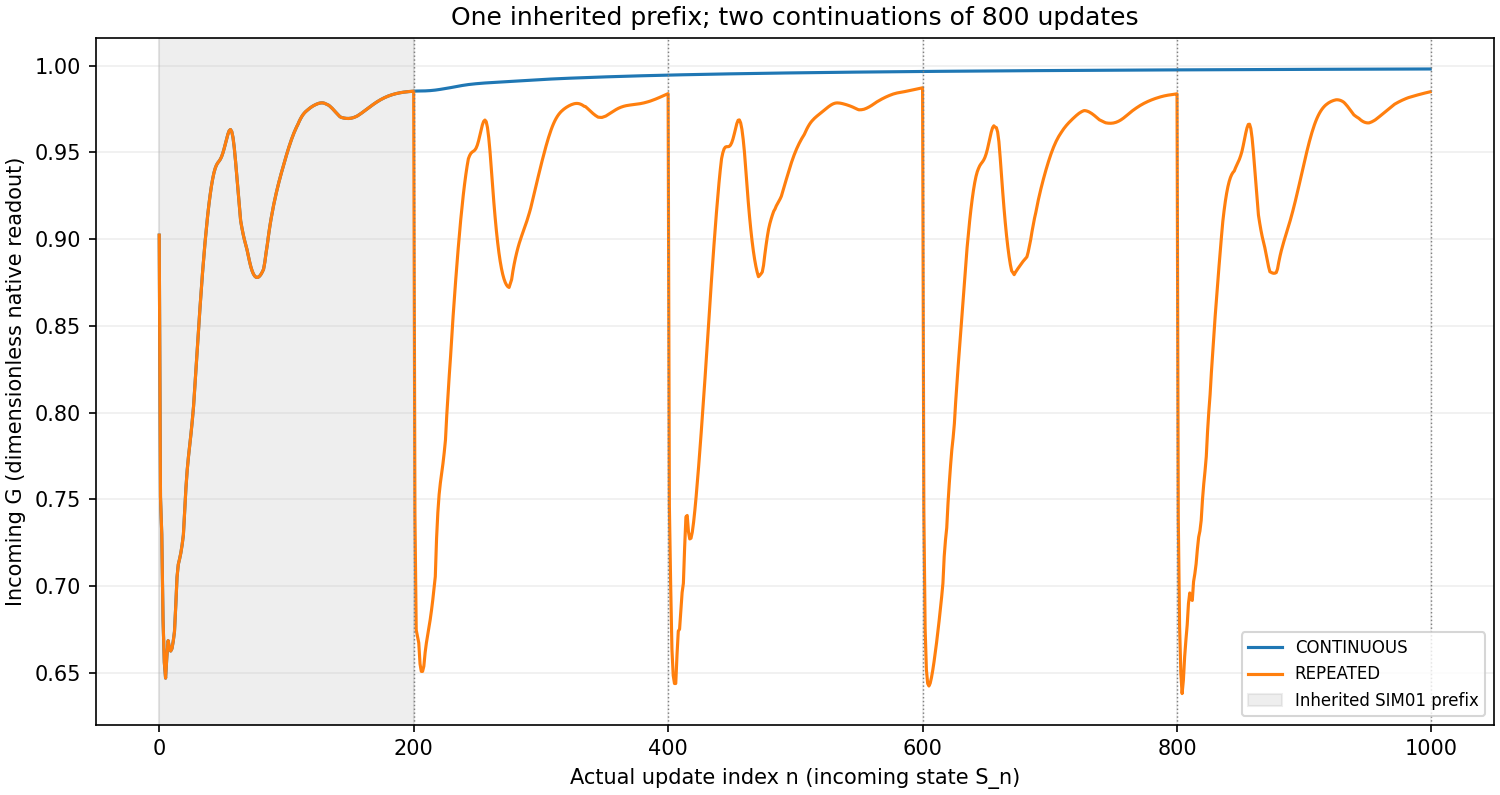
\includegraphics[width=.93\linewidth]{03_incoming_G.png}
\caption{Incoming G at actual update $n$, from state $S_n$. The shaded first 200 updates are the single inherited cycle 0. The later four blocks are new; only REPEATED resets its supplied frame at their boundaries. G remained above 0.5 in both arms. Unchanged accepted figure~\cite{sim02,records}.}
\label{fig:G-actual}
\end{figure}

\begin{figure}[!htbp]
\centering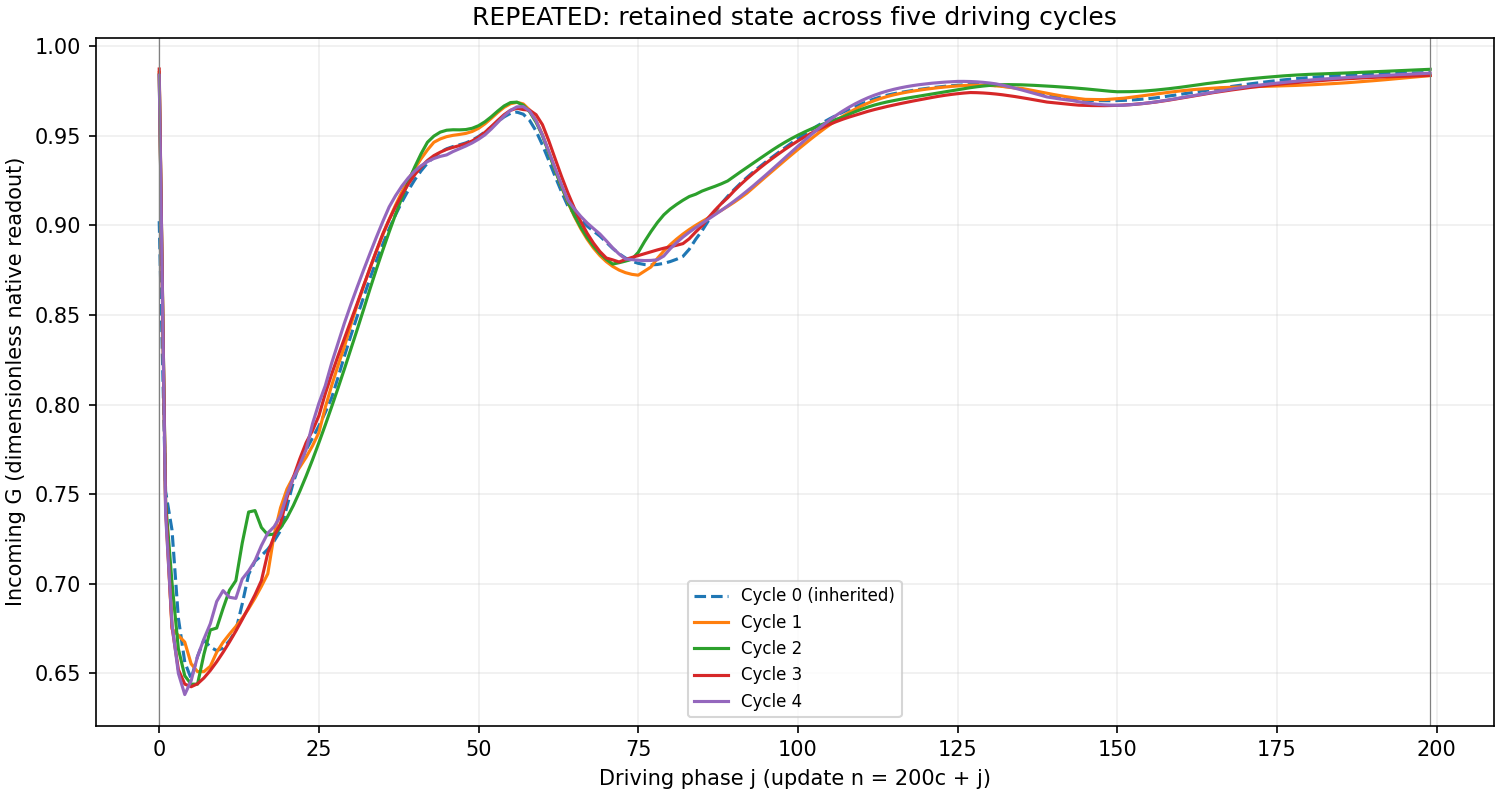
\includegraphics[width=.93\linewidth]{06_repeated_G.png}
\caption{REPEATED incoming G at phase $j$ of update $200c+j$, evaluated from $S_{200c+j}$. Dashed cycle 0 is inherited; cycles 1--4 are newly executed. The state and RNG continue across phase resets. Unchanged accepted figure~\cite{sim02,records}.}
\label{fig:G-phase}
\end{figure}
\end{document}
